\section{Opis projektu ,,Karta Pacjenta''}
Projekt ,,Karta Pacjenta'' zakładał stworzenie aplikacji umożliwiającej przechowywanie danych pacjentów w serwisie bazodanowym. Aplikacja przechowuje informacje dotyczące chorób przebytych przez pacjenta, wystawionych przez lekarza recept. Umożliwia bezpieczne przechowywanie danych wrażliwych, takich jak pesel, numer telefonu itd. Umożliwia także prezentację tych danych oraz ich eksport (także w postaci anonimowej - bez danych osobowych - posiadających tylko informację o przebytej chorobie, nie o pacjencie). 

Aplikacja powstała przy użyciu języków: Java (ang. \textit{backend}) oraz Angular (TypeScript) (ang. \textit{frontend}). Serwis postawiony jest na darmowej domenie dostępnej pod \href{http://trunk-kartapacjenta.herokuapp.com/}{tym linkiem}. Gorąco zachęcamy do zapoznania się z działaniem aplikacji. 

Dzięki serwisowi \href{https://heroku.com/} {Heroku} możliwe było darmowe opublikowanie witryny w internecie. Nawet w darmowej wersji serwis ten zapewnia usługi związane z CI (ang. \textit{Continuous Integration}). Efektem tego, jest fakt, że po każdej aktualizacji zdalnego repozytorium \textit{Git} serwis automatycznie przebudowuje się.

\subsection{Przedstawienie aplikacji}

% login page
\begin{figure}[H]
\centering
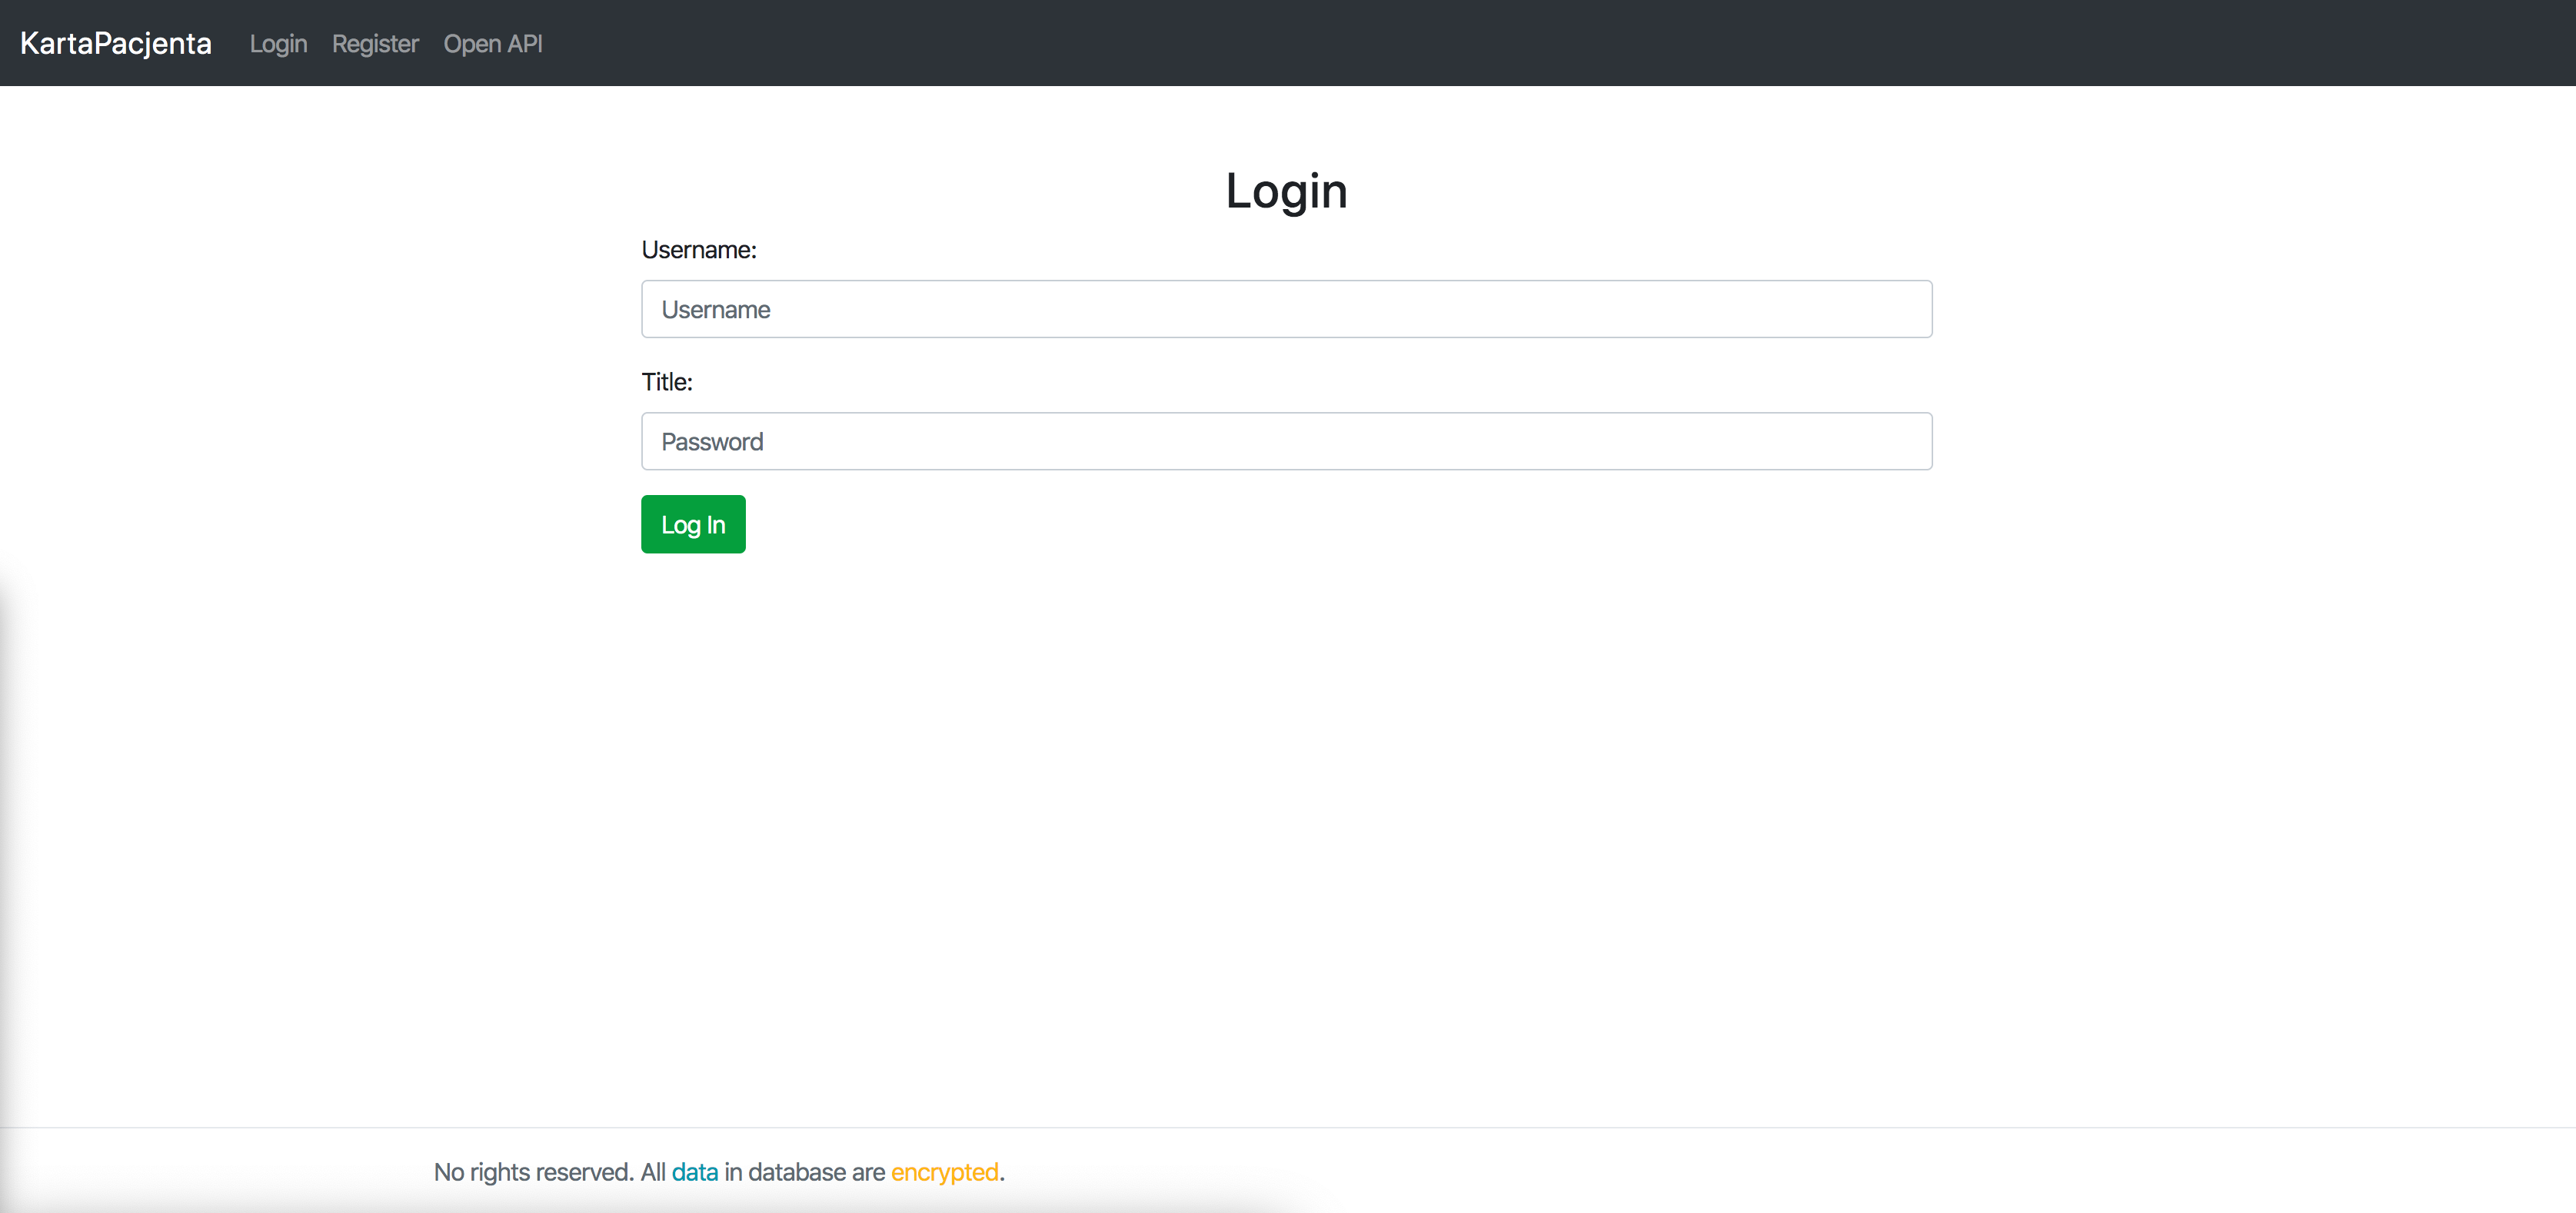
\includegraphics[width=15cm]{pictures/service/01_login}
\caption{Przedstawienie ekranu logowania.}
\end{figure}

% admin panel
\begin{figure}[H]
\centering
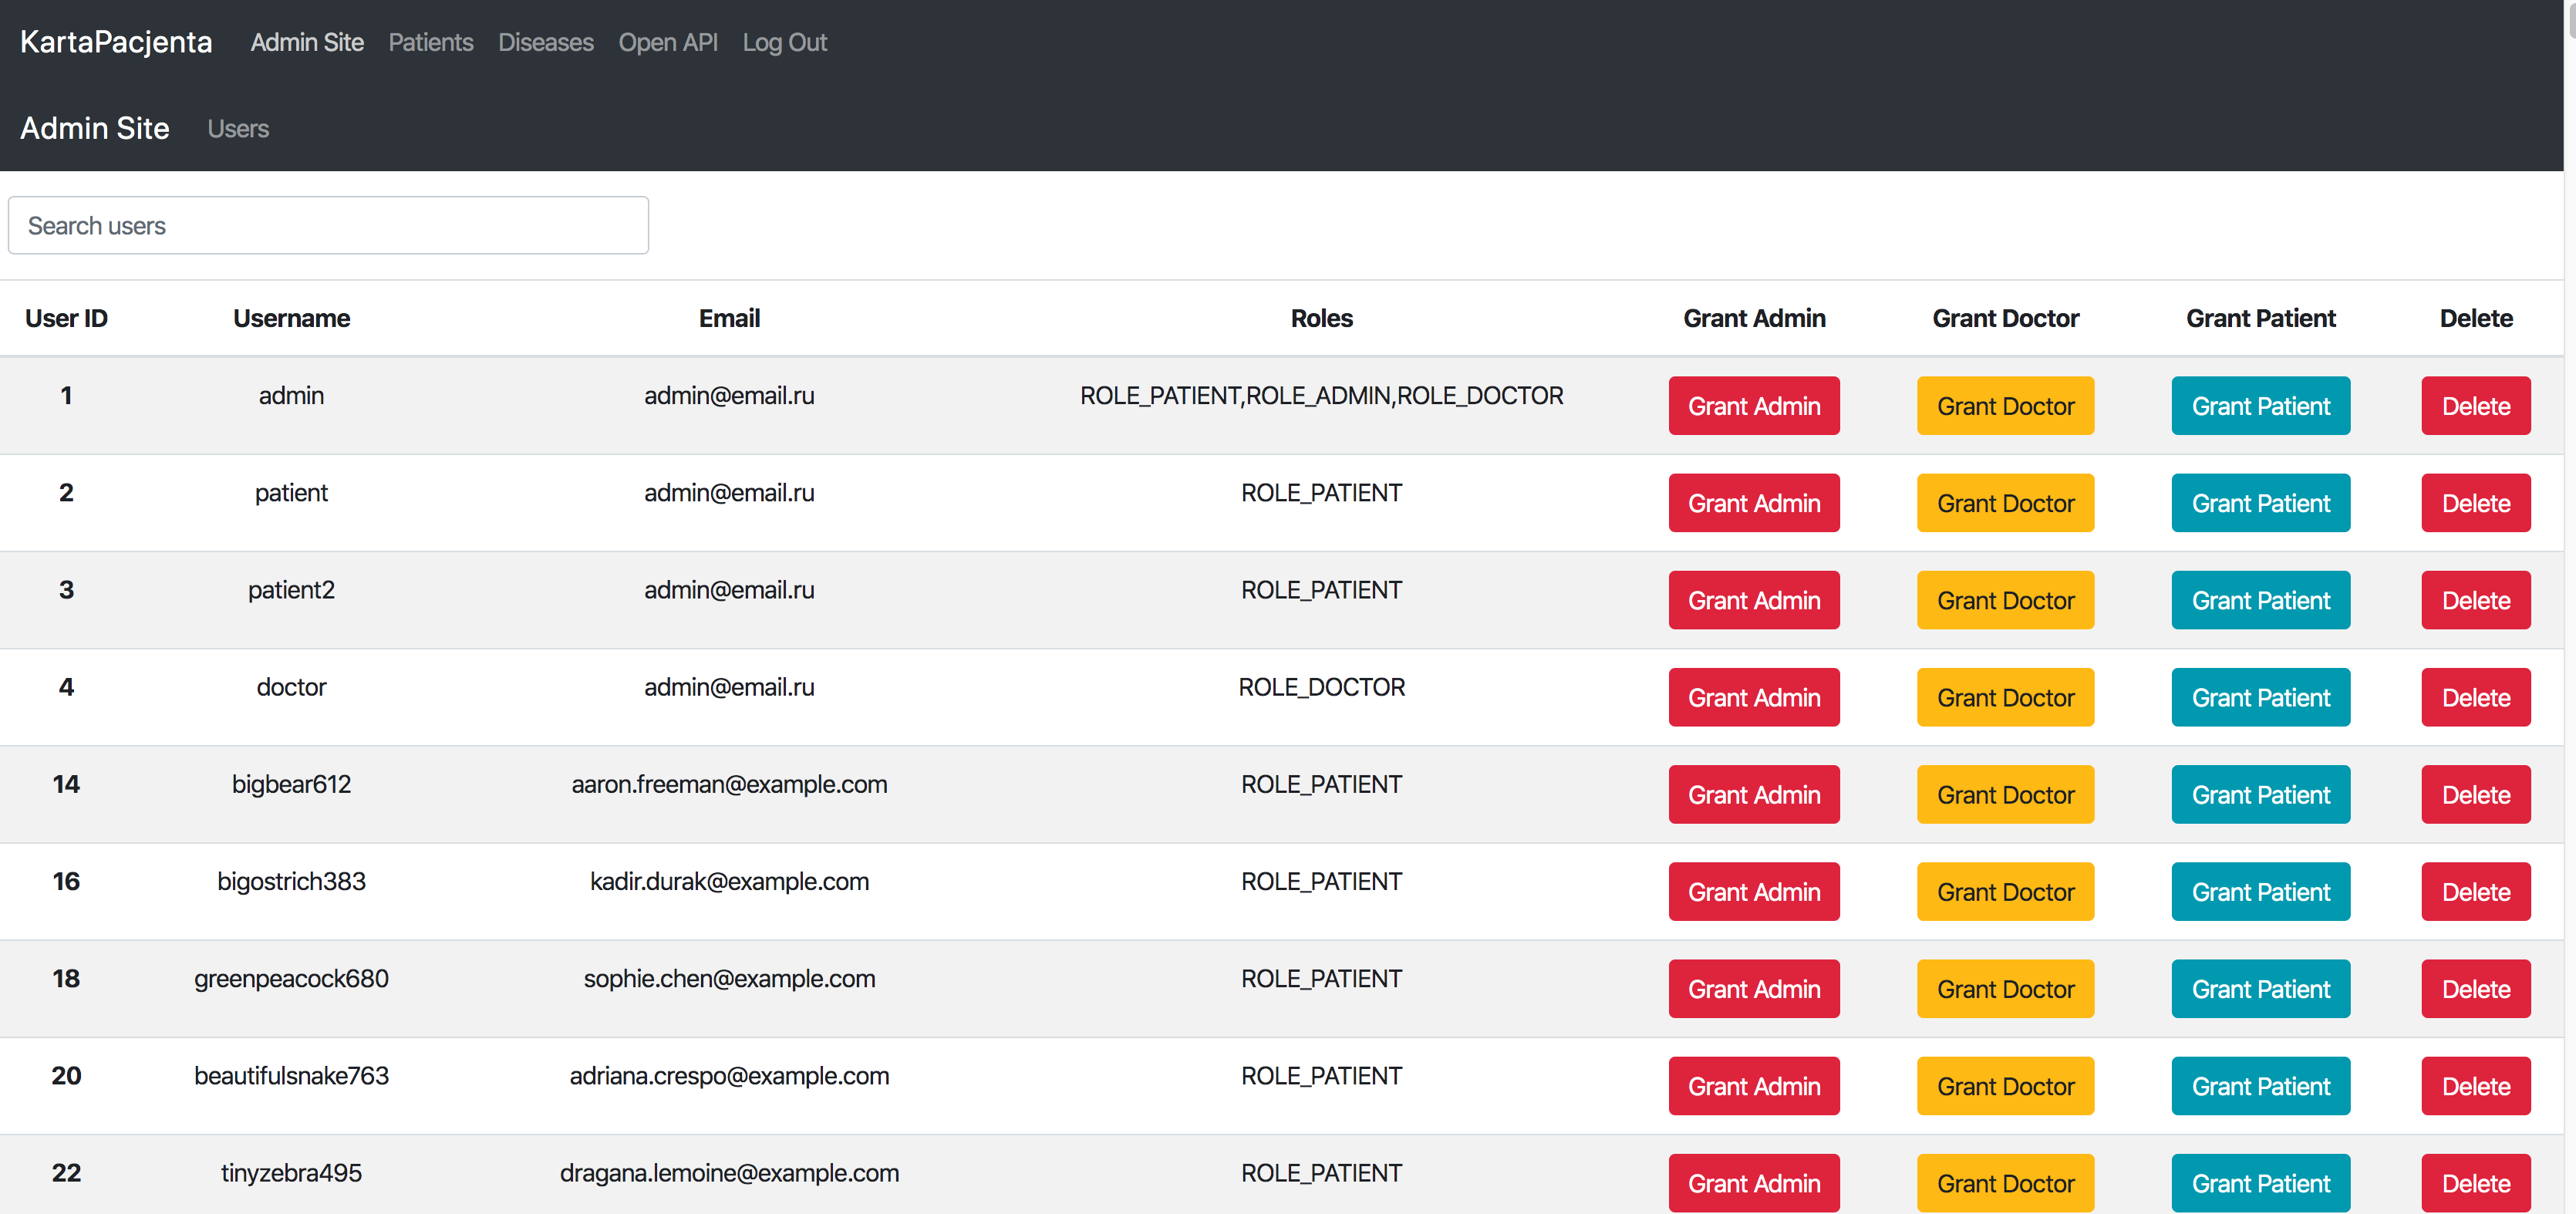
\includegraphics[width=15cm]{pictures/service/02-admin_panel}
\caption{Przedstawienie panelu administratora, umożliwiającego nadawanie praw, oraz usuwanie użytkowników.}
\end{figure}

% choroby
\begin{figure}[H]
\centering
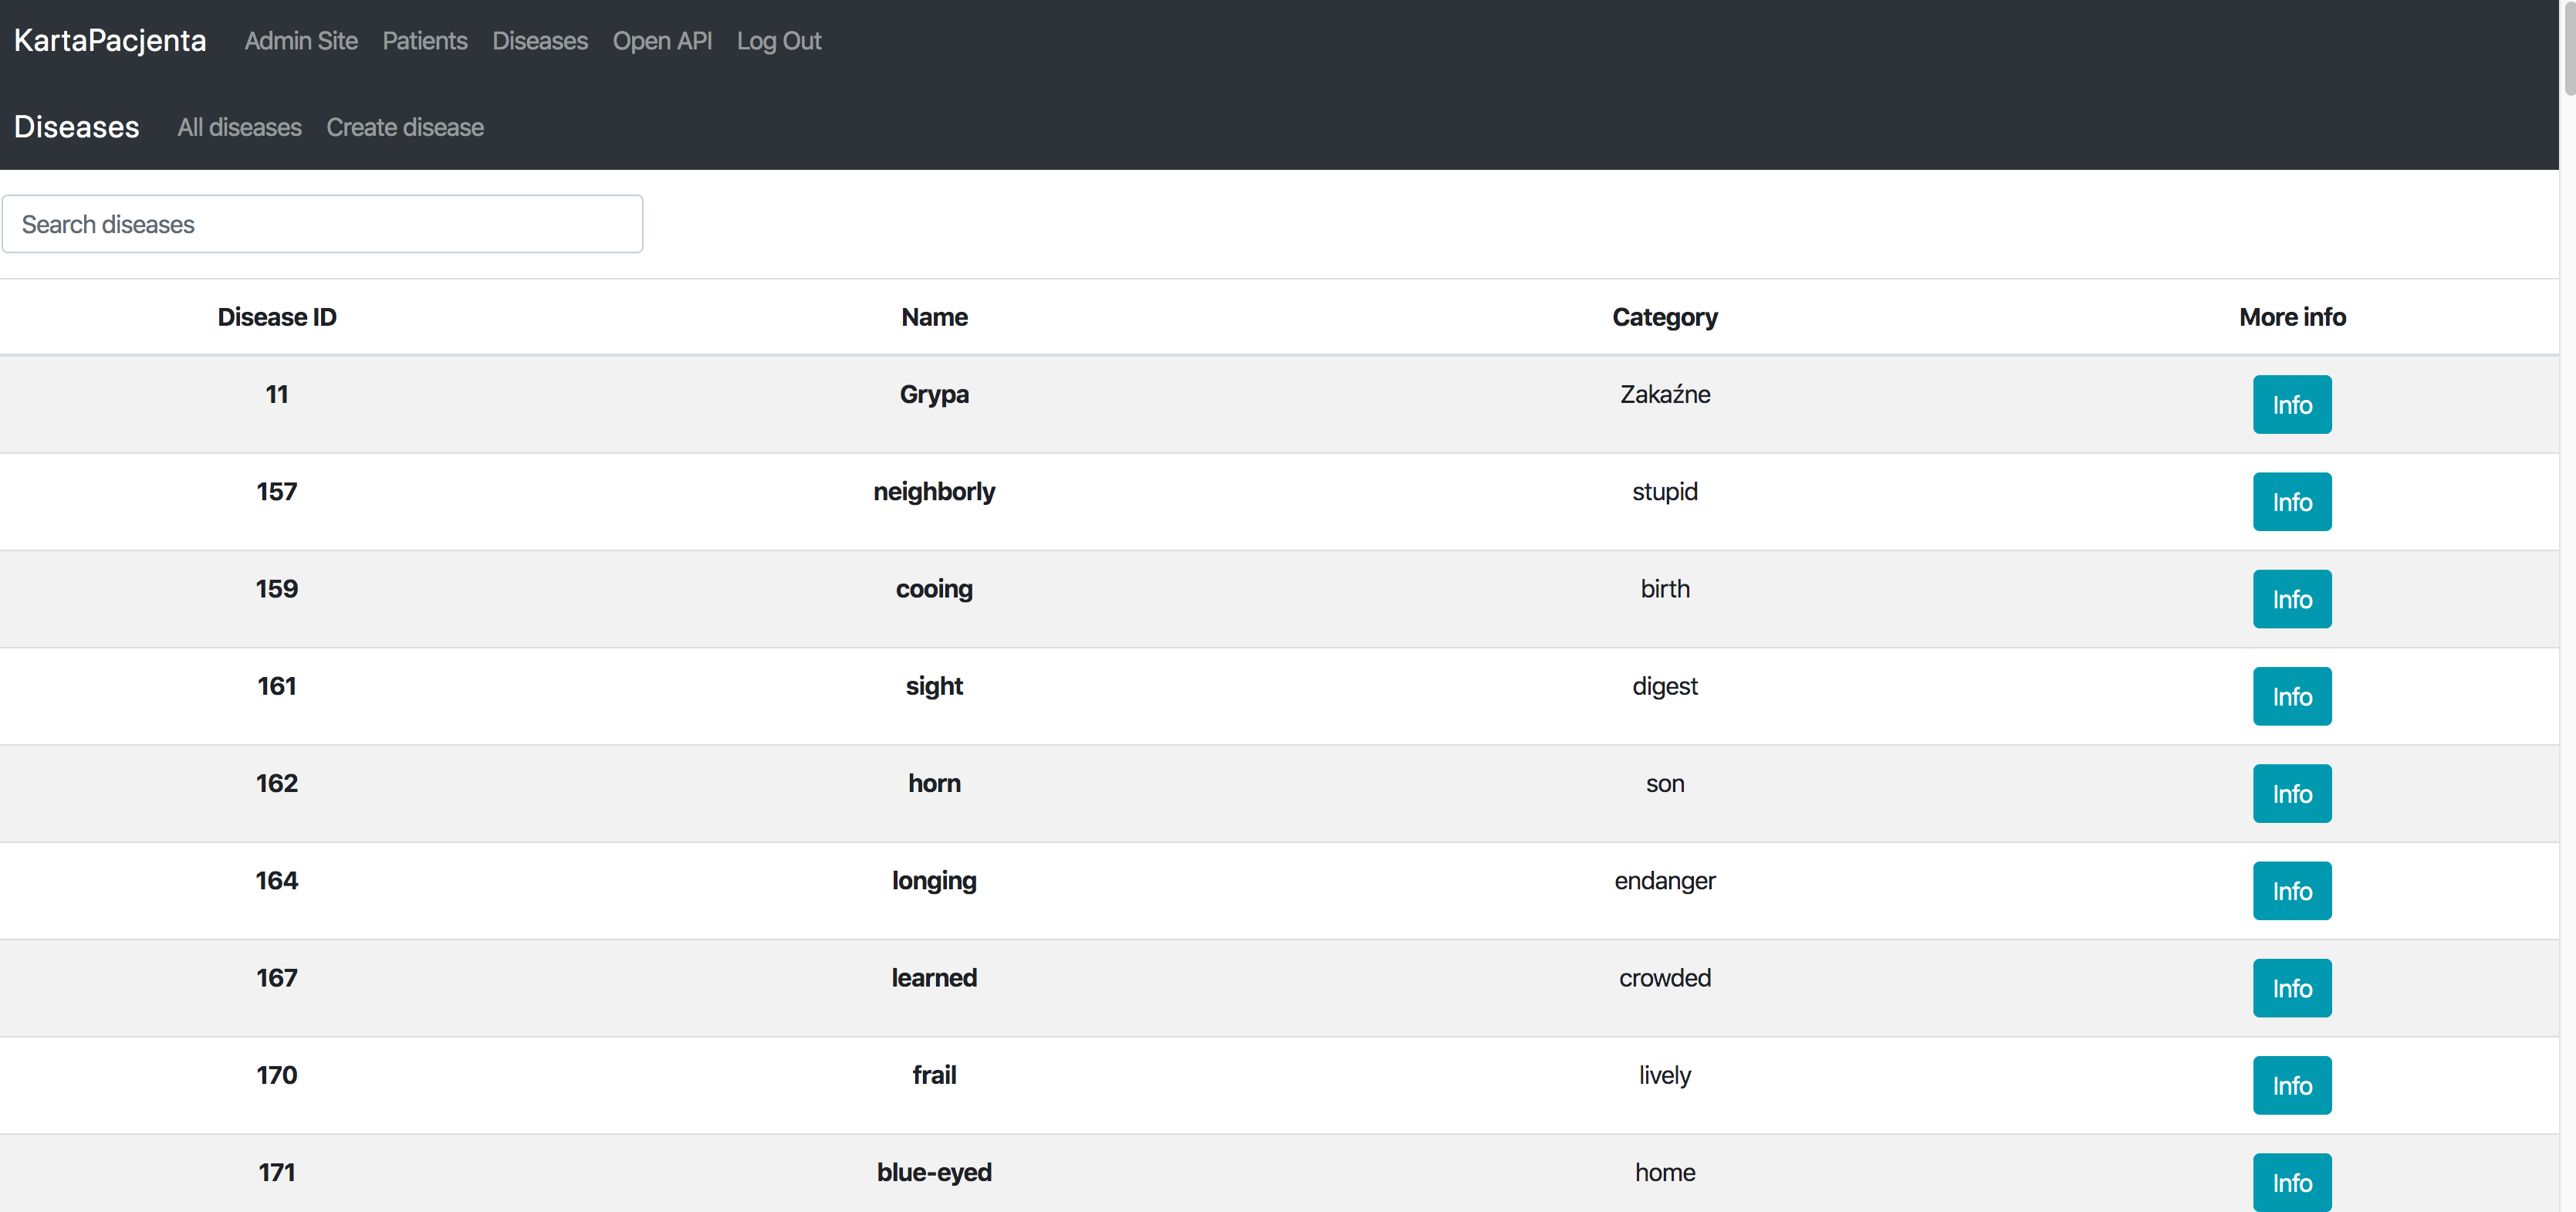
\includegraphics[width=15cm]{pictures/service/04-choroby}
\caption{Przedstawienie zakładki zawierającej wypisane wszystkie zapisane w systemie choroby. Obok widoczna zakładka umożliwiająca dodanie nowej choroby. Przycisk \textit{,,info''} w tabeli \textit{,,More info''} umożliwia zapoznanie się z dostępnymi informacjami dotyczącymi danej choroby.}
\end{figure}

% patients
\begin{figure}[H]
\centering
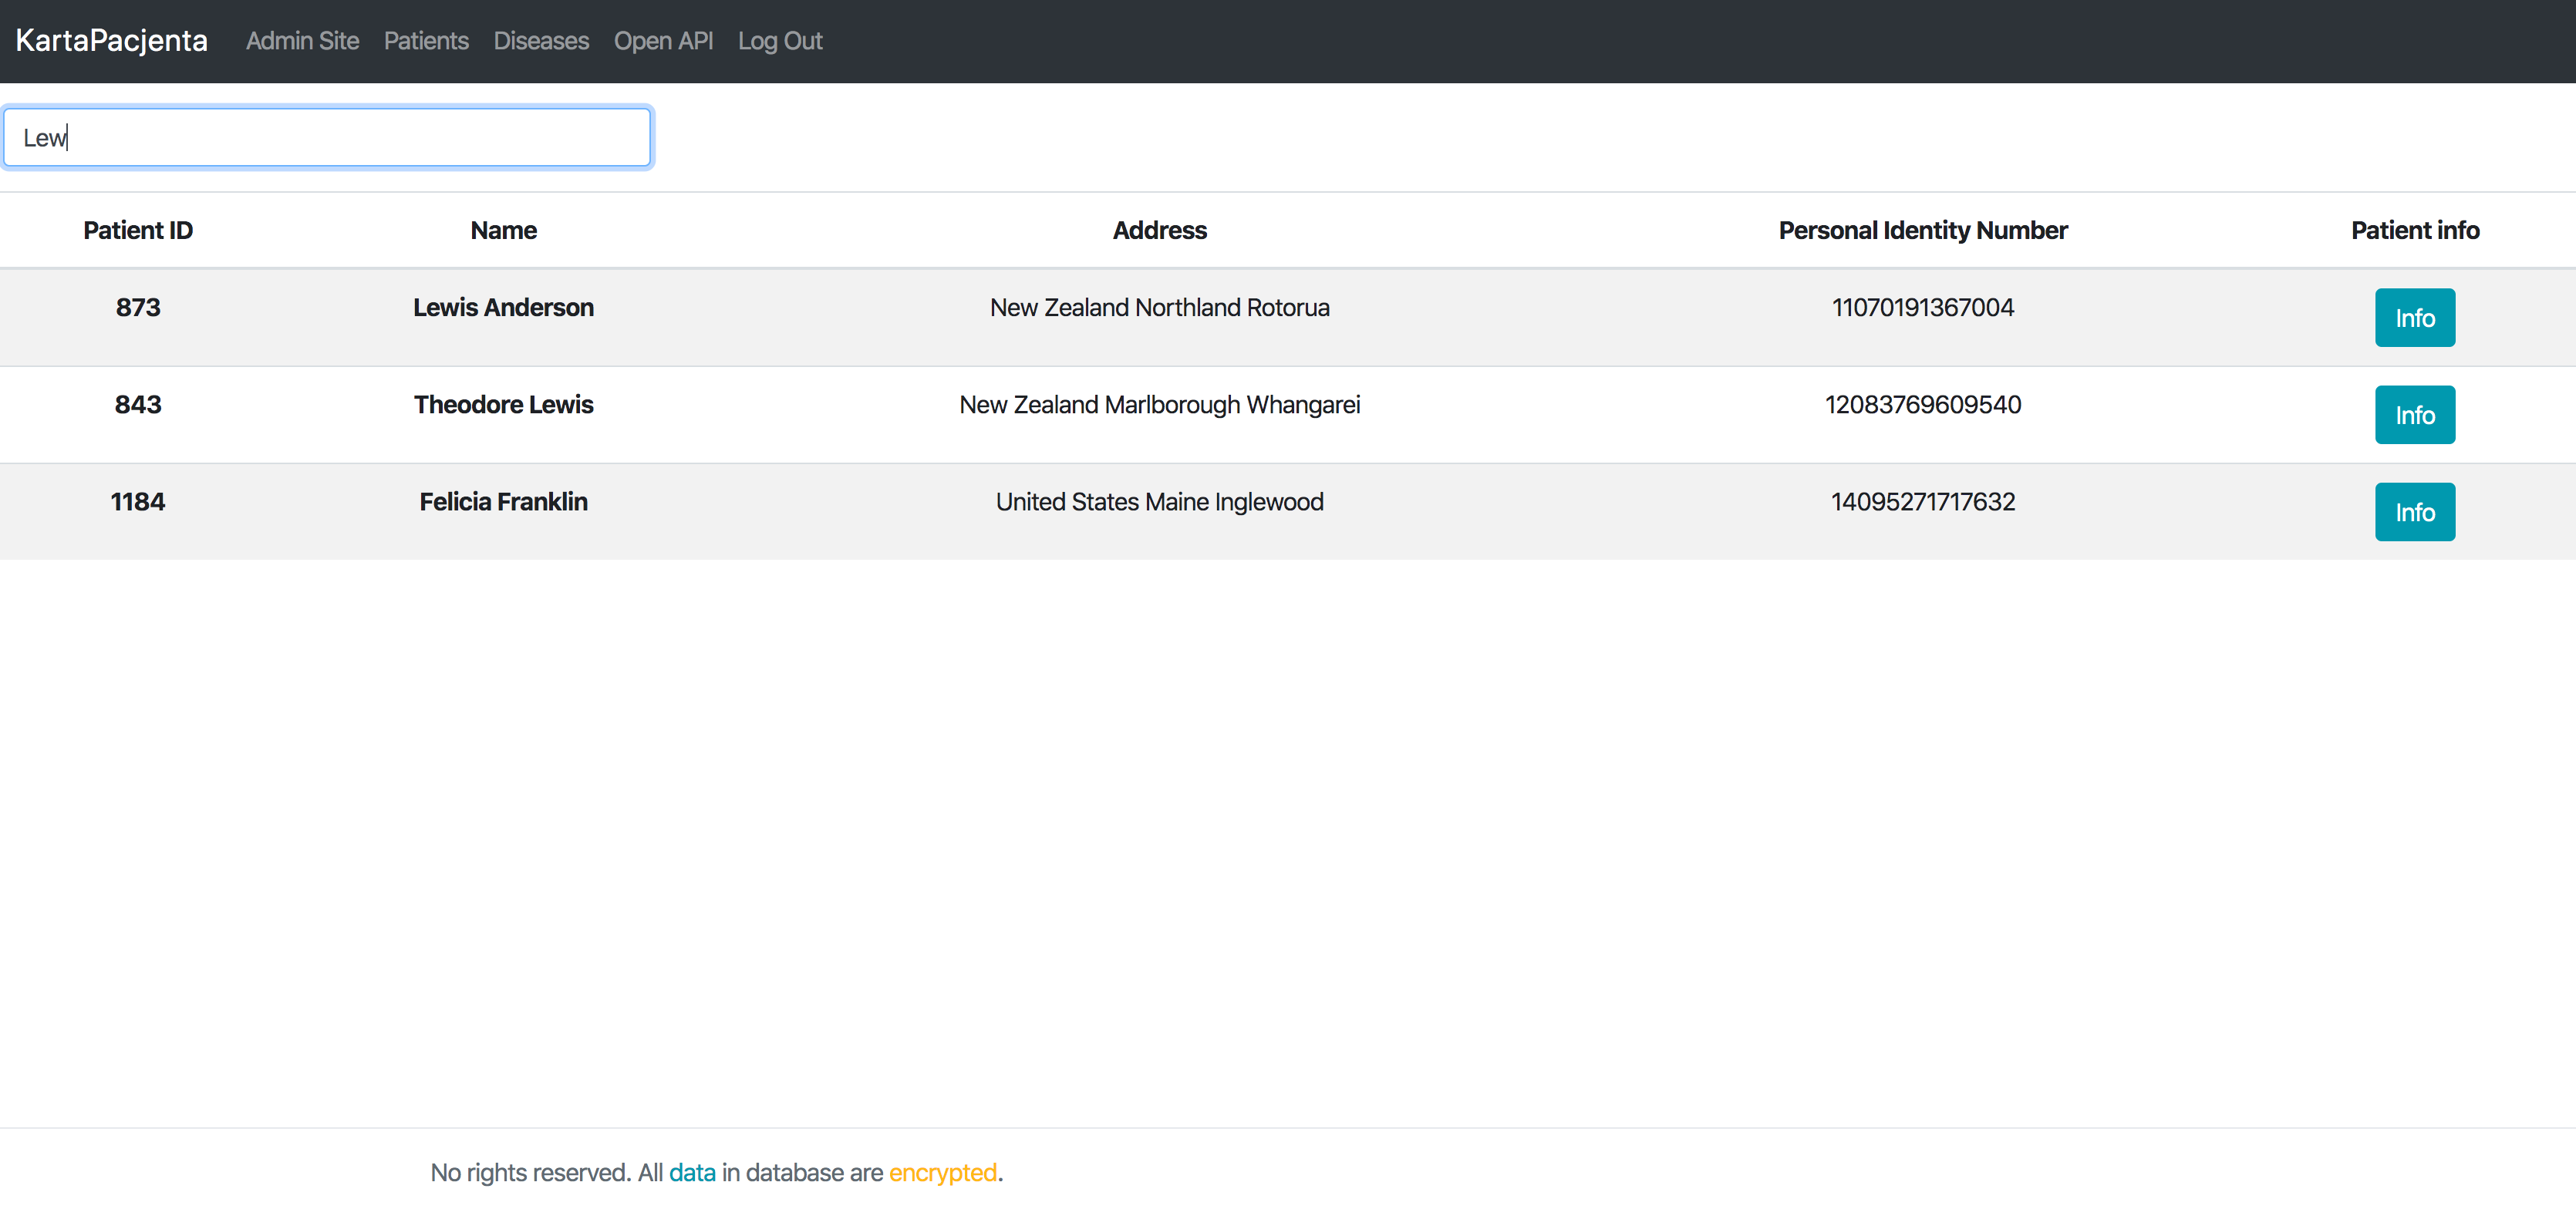
\includegraphics[width=15cm]{pictures/service/03-patients}
\caption{Przedstawienie zakładki zawierającej wszystkich dostępnych pacjentów. Na zdjęciu przedstawiona jest możliwość filtracji pacjentów.}
\end{figure}

%patient-ingo
\begin{figure}[H]
\centering
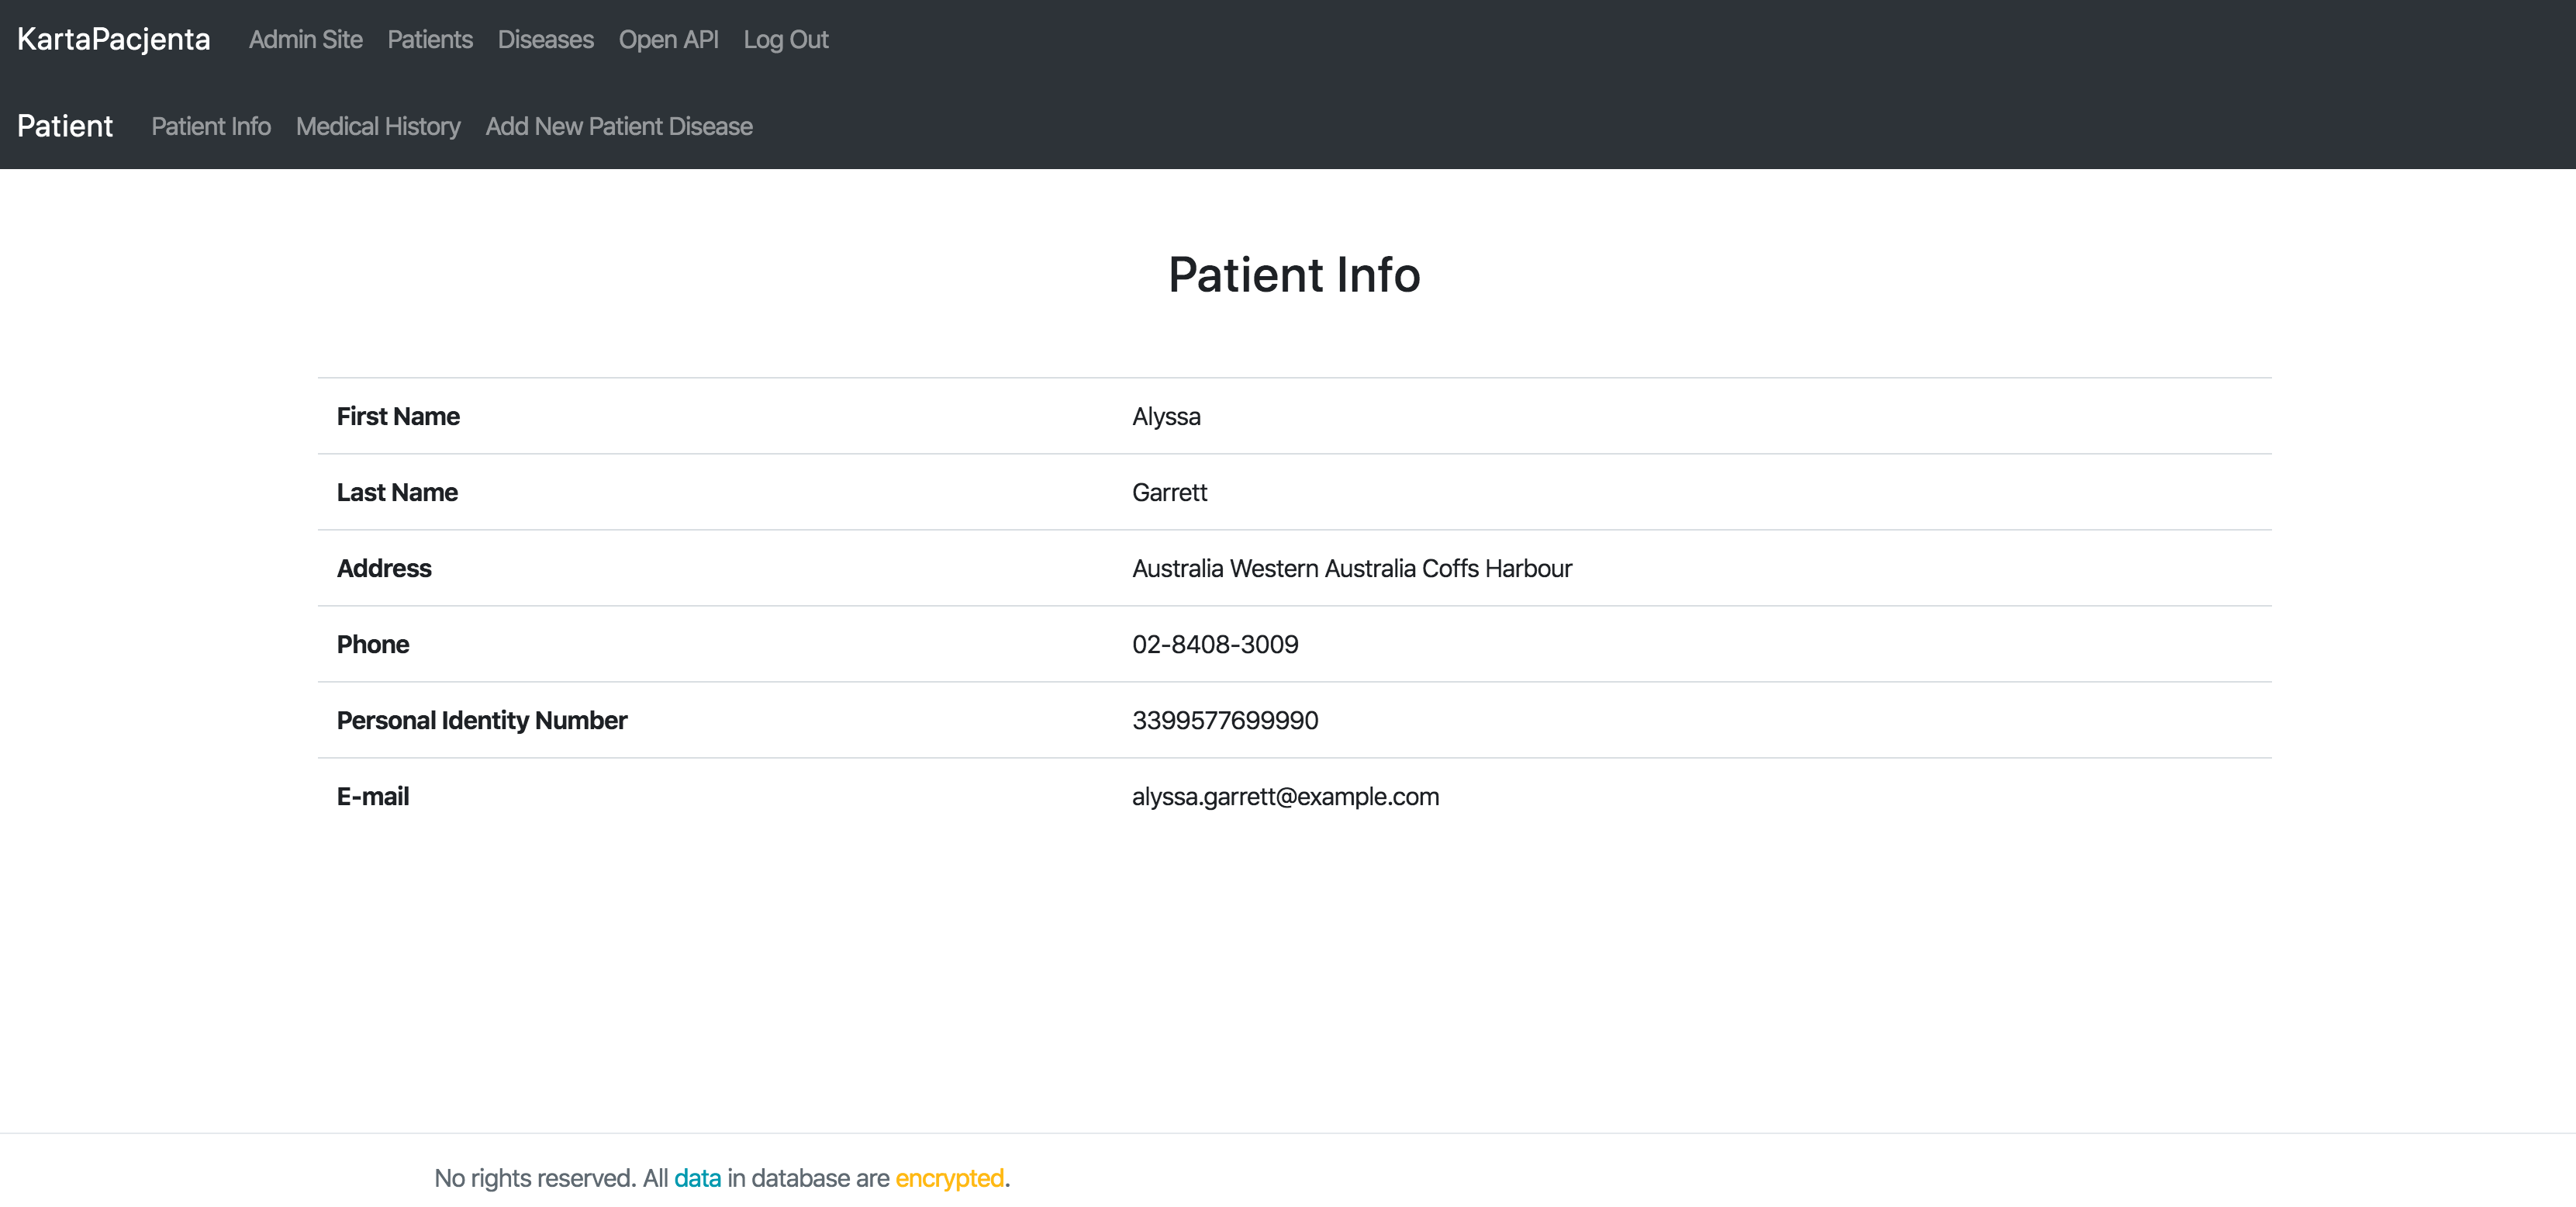
\includegraphics[width=15cm]{pictures/service/05-patient_info}
\caption{Przedstawienie zakładki zawierającej informacje o wybranym pacjencie.}
\end{figure}

% choroby pacjenta
\begin{figure}[H]
\centering
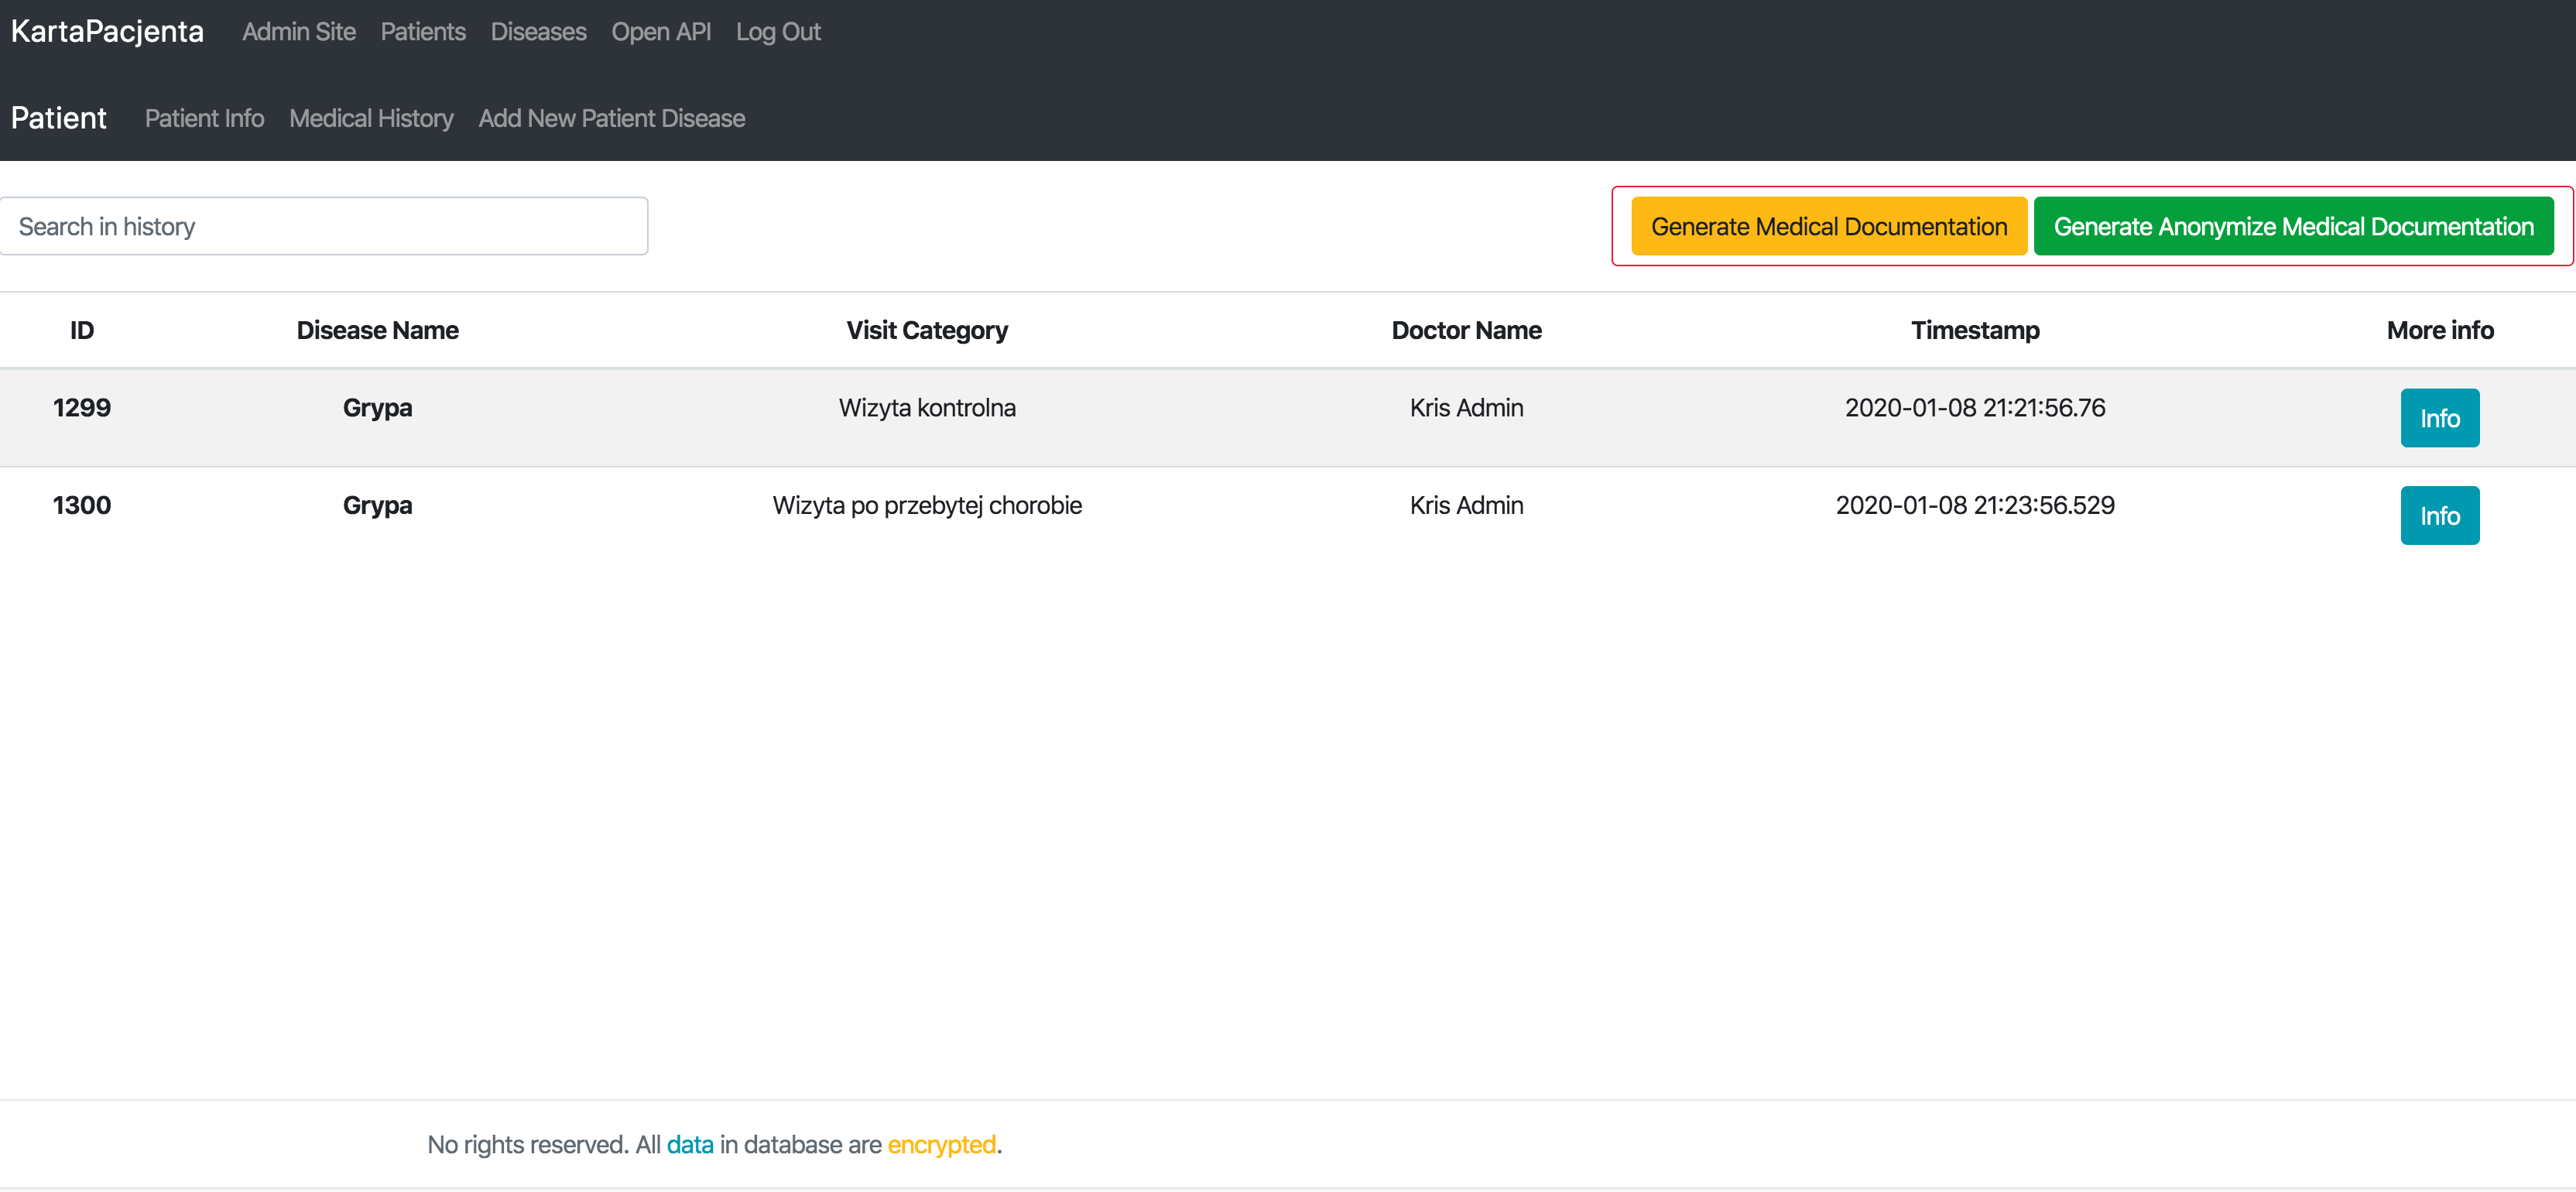
\includegraphics[width=15cm]{pictures/service/06-choroby_pacjenta}
\caption{Przedstawienie zakładki zawierającej informacje dotyczące przebytych przez pacjenta wizytach u doktora wraz z informacją jakiej choroby konkretna wizyta dotyczyła.}
\end{figure}

% historia normalna
\begin{figure}[H]
\centering
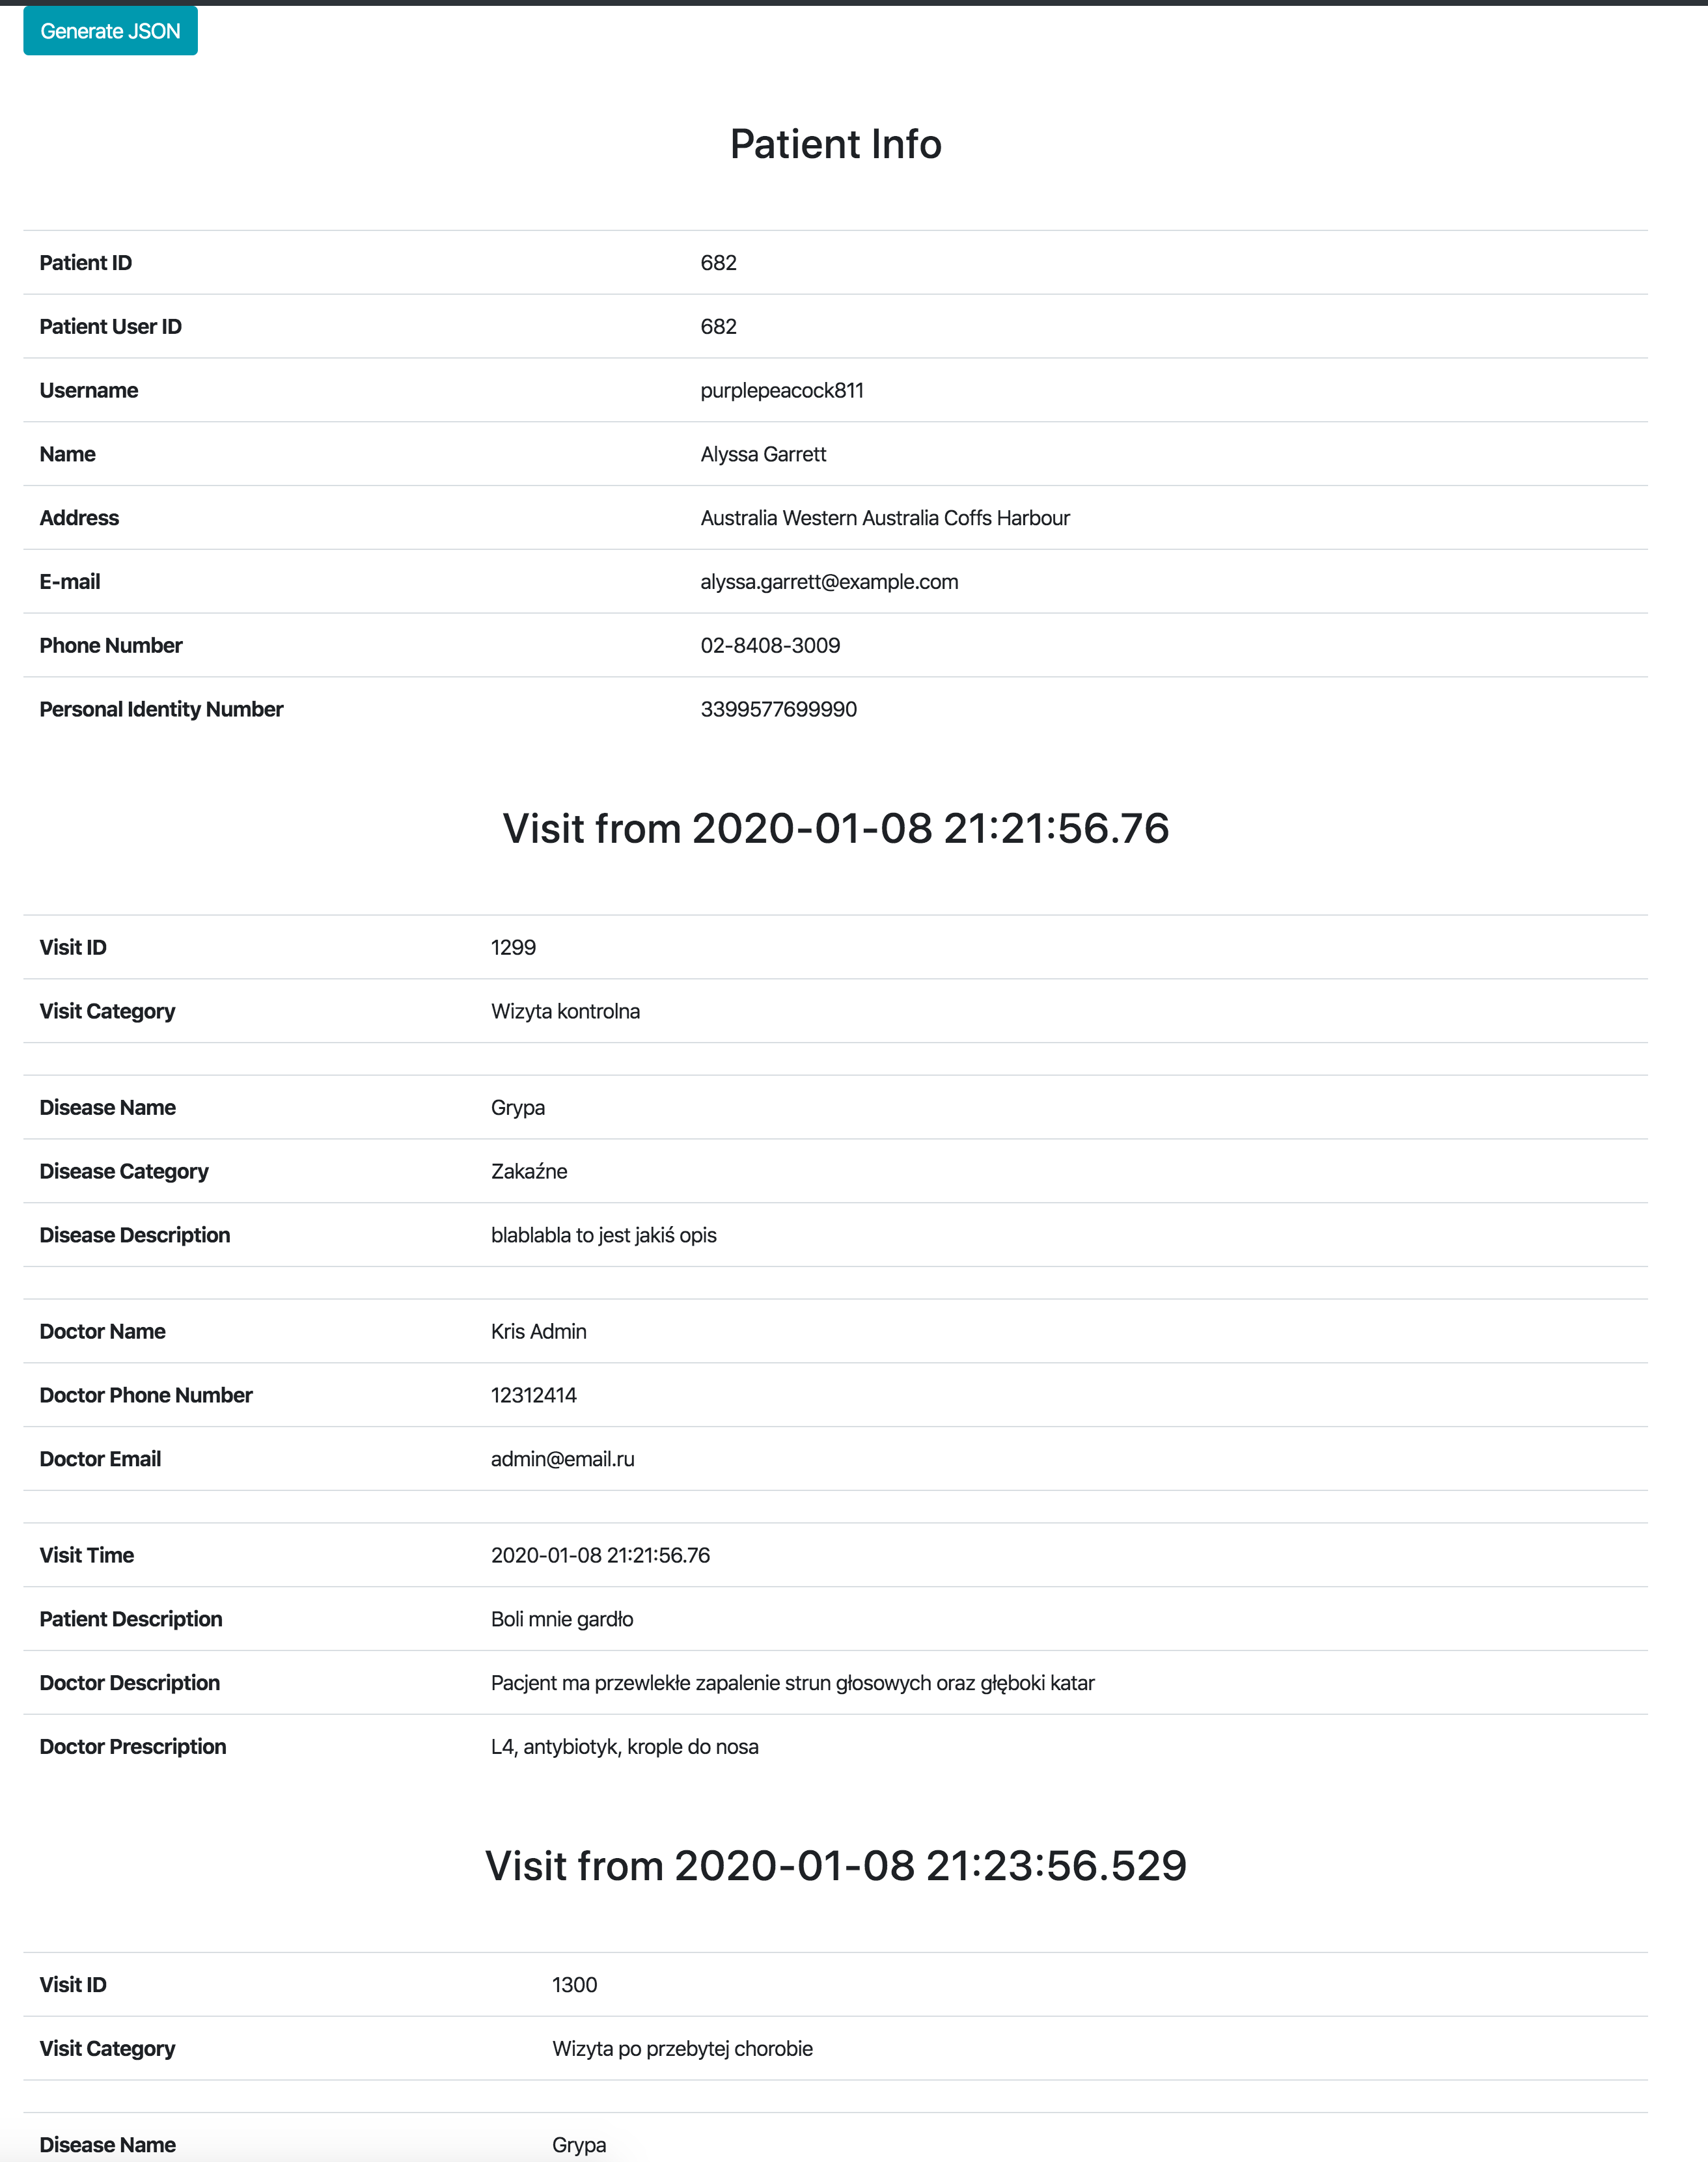
\includegraphics[width=15cm]{pictures/service/09-history_normal}
\caption{Przedstawienie zakładki zawierającej pełną historię przebytych chorób, dotyczącą konkretnego pacjenta. Zakładka dostępna jest dla lekarza (dla wszystkich pacjentów). Pacjent ma dostęp wyłącznie do swojej prywatnej historii chorób.}
\end{figure}

% histora anonimowa
\begin{figure}[H]
\centering
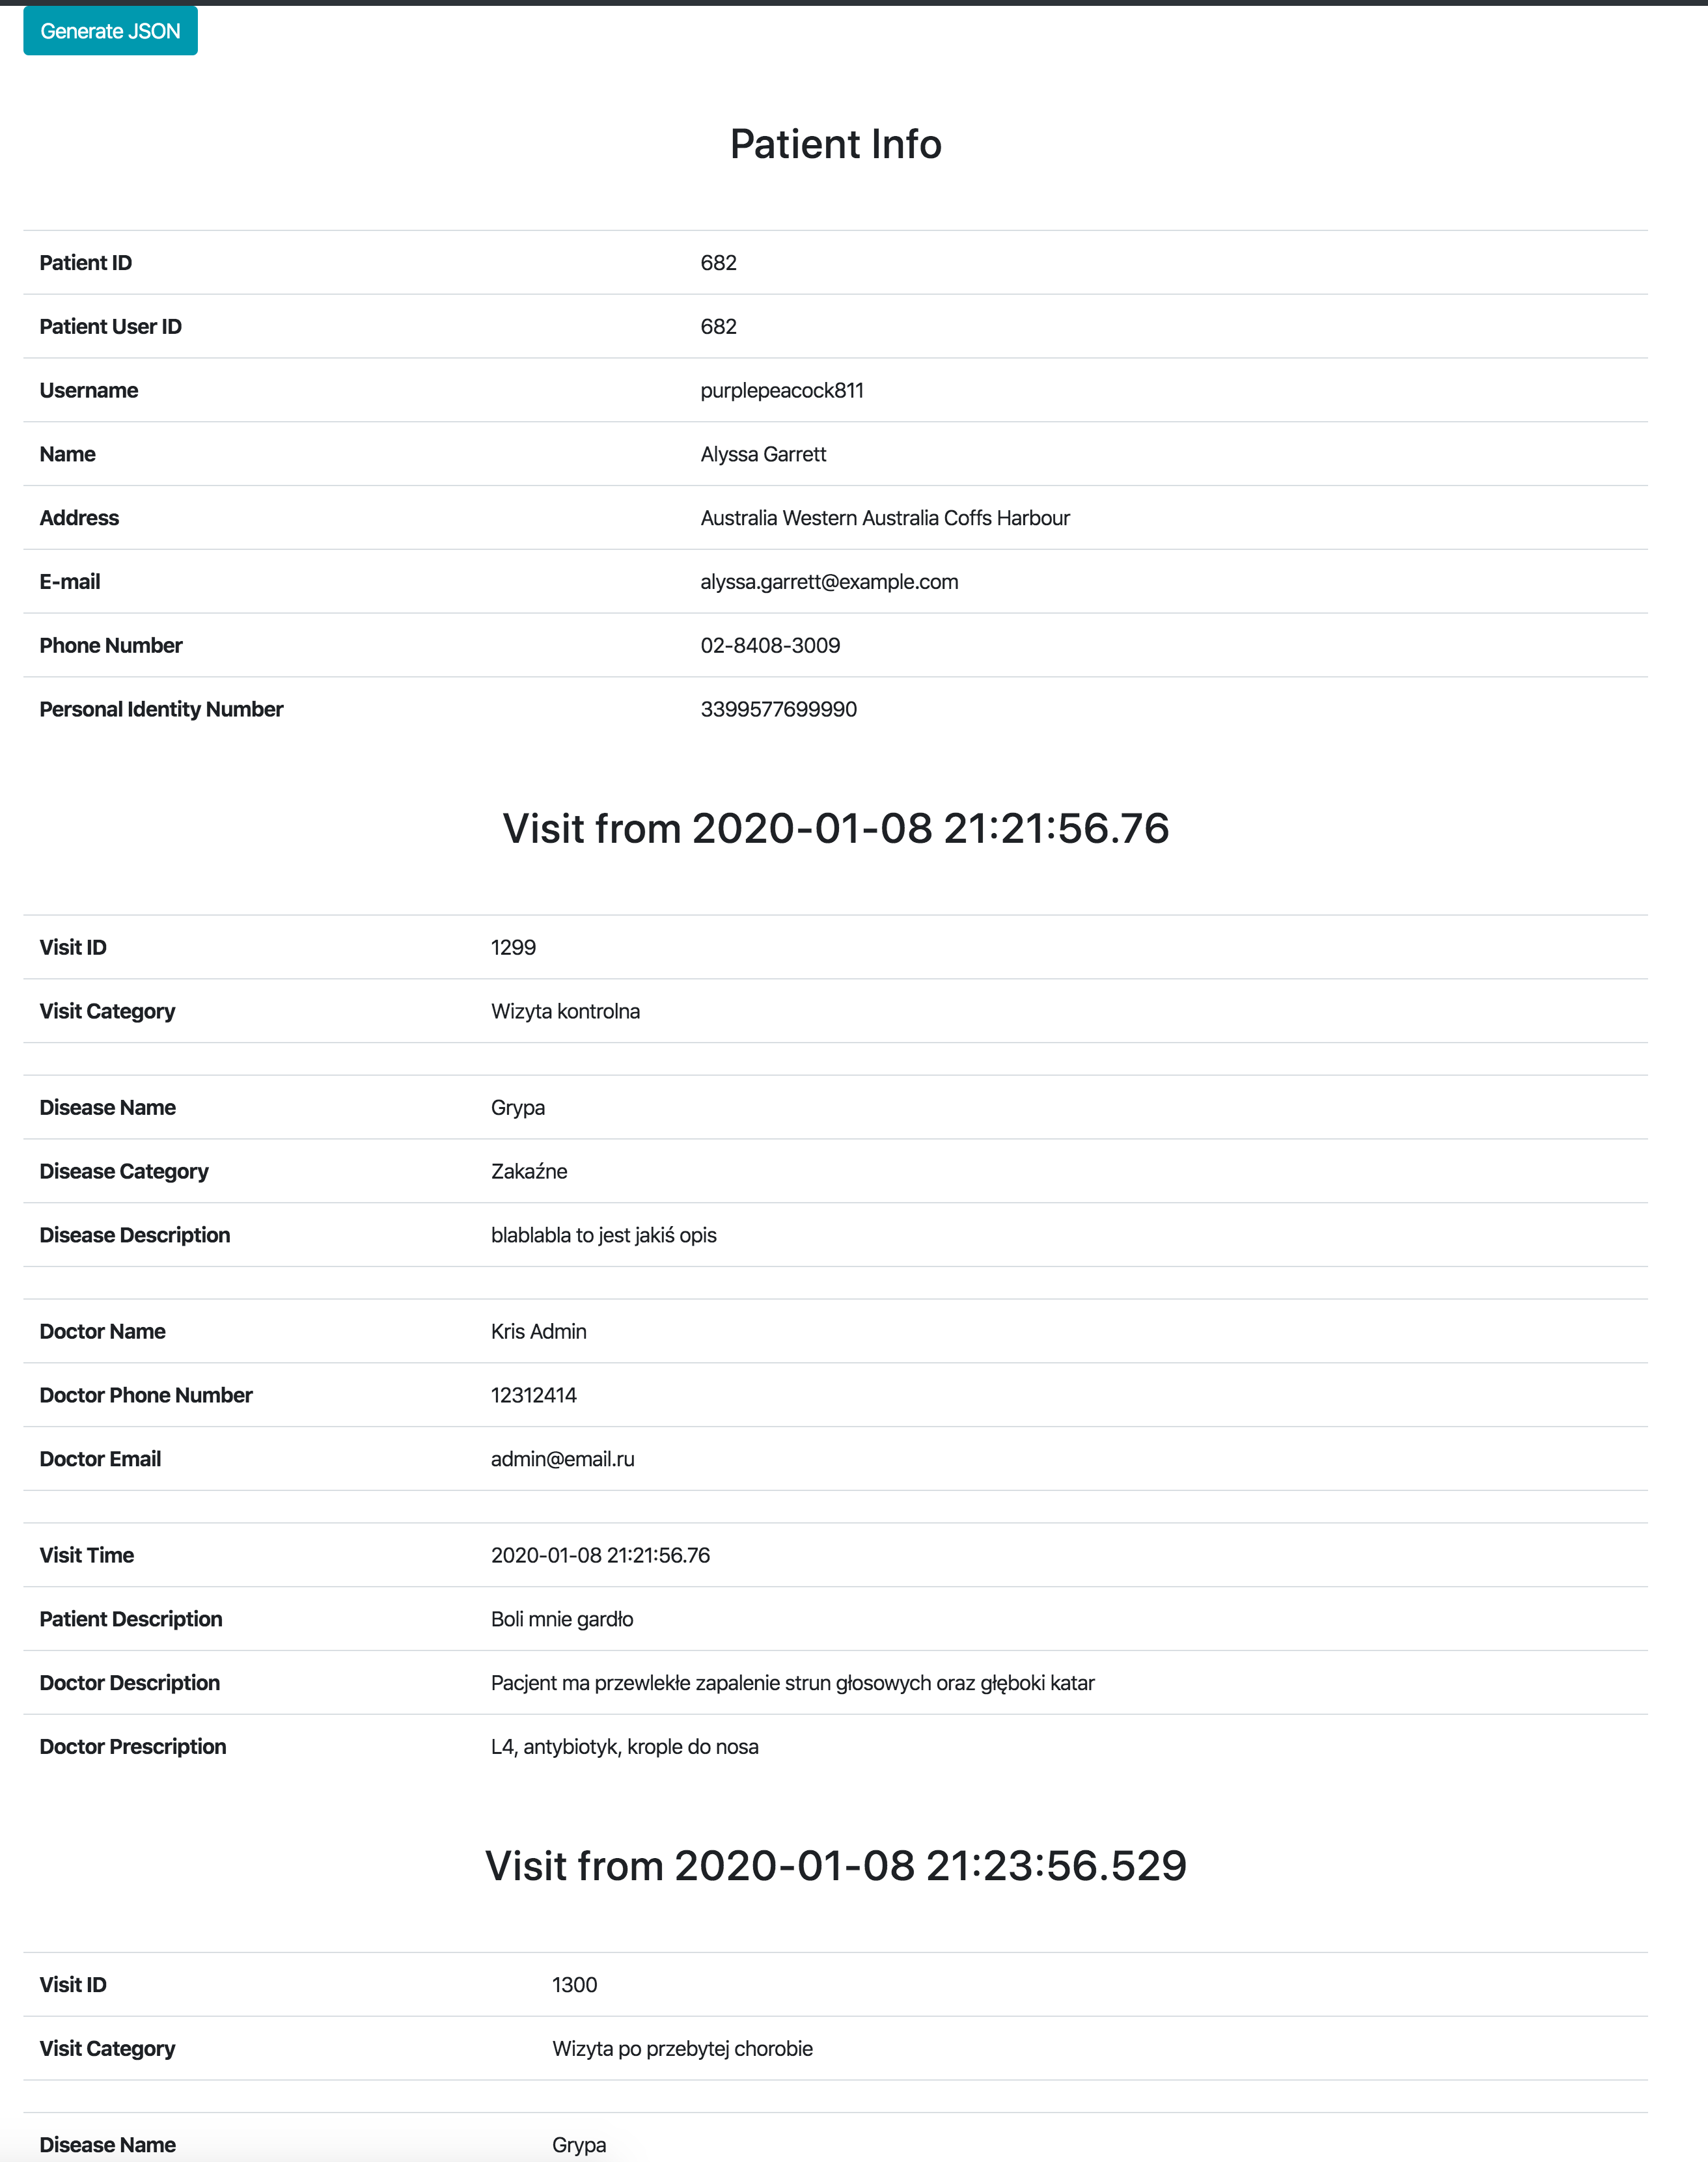
\includegraphics[width=15cm]{pictures/service/09-history_normal}
\caption{Przedstawienie zakładki zawierającej anonimową historię pacjenta - brak w niej danych wrażliwych umożliwiających identyfikację pacjenta.}
\label{history_pic}
\end{figure}

% json normal
Serwis umożliwia wygenerowanie danych o pacjencie i przebytych chorobach w zunifikowanym formacie \textit{JSON}. Jest to możliwe na stronie związanej w historią choroby pacjenta, przedstawionej na rysunku \ref{history_pic}.
\begin{figure}[H]
\centering
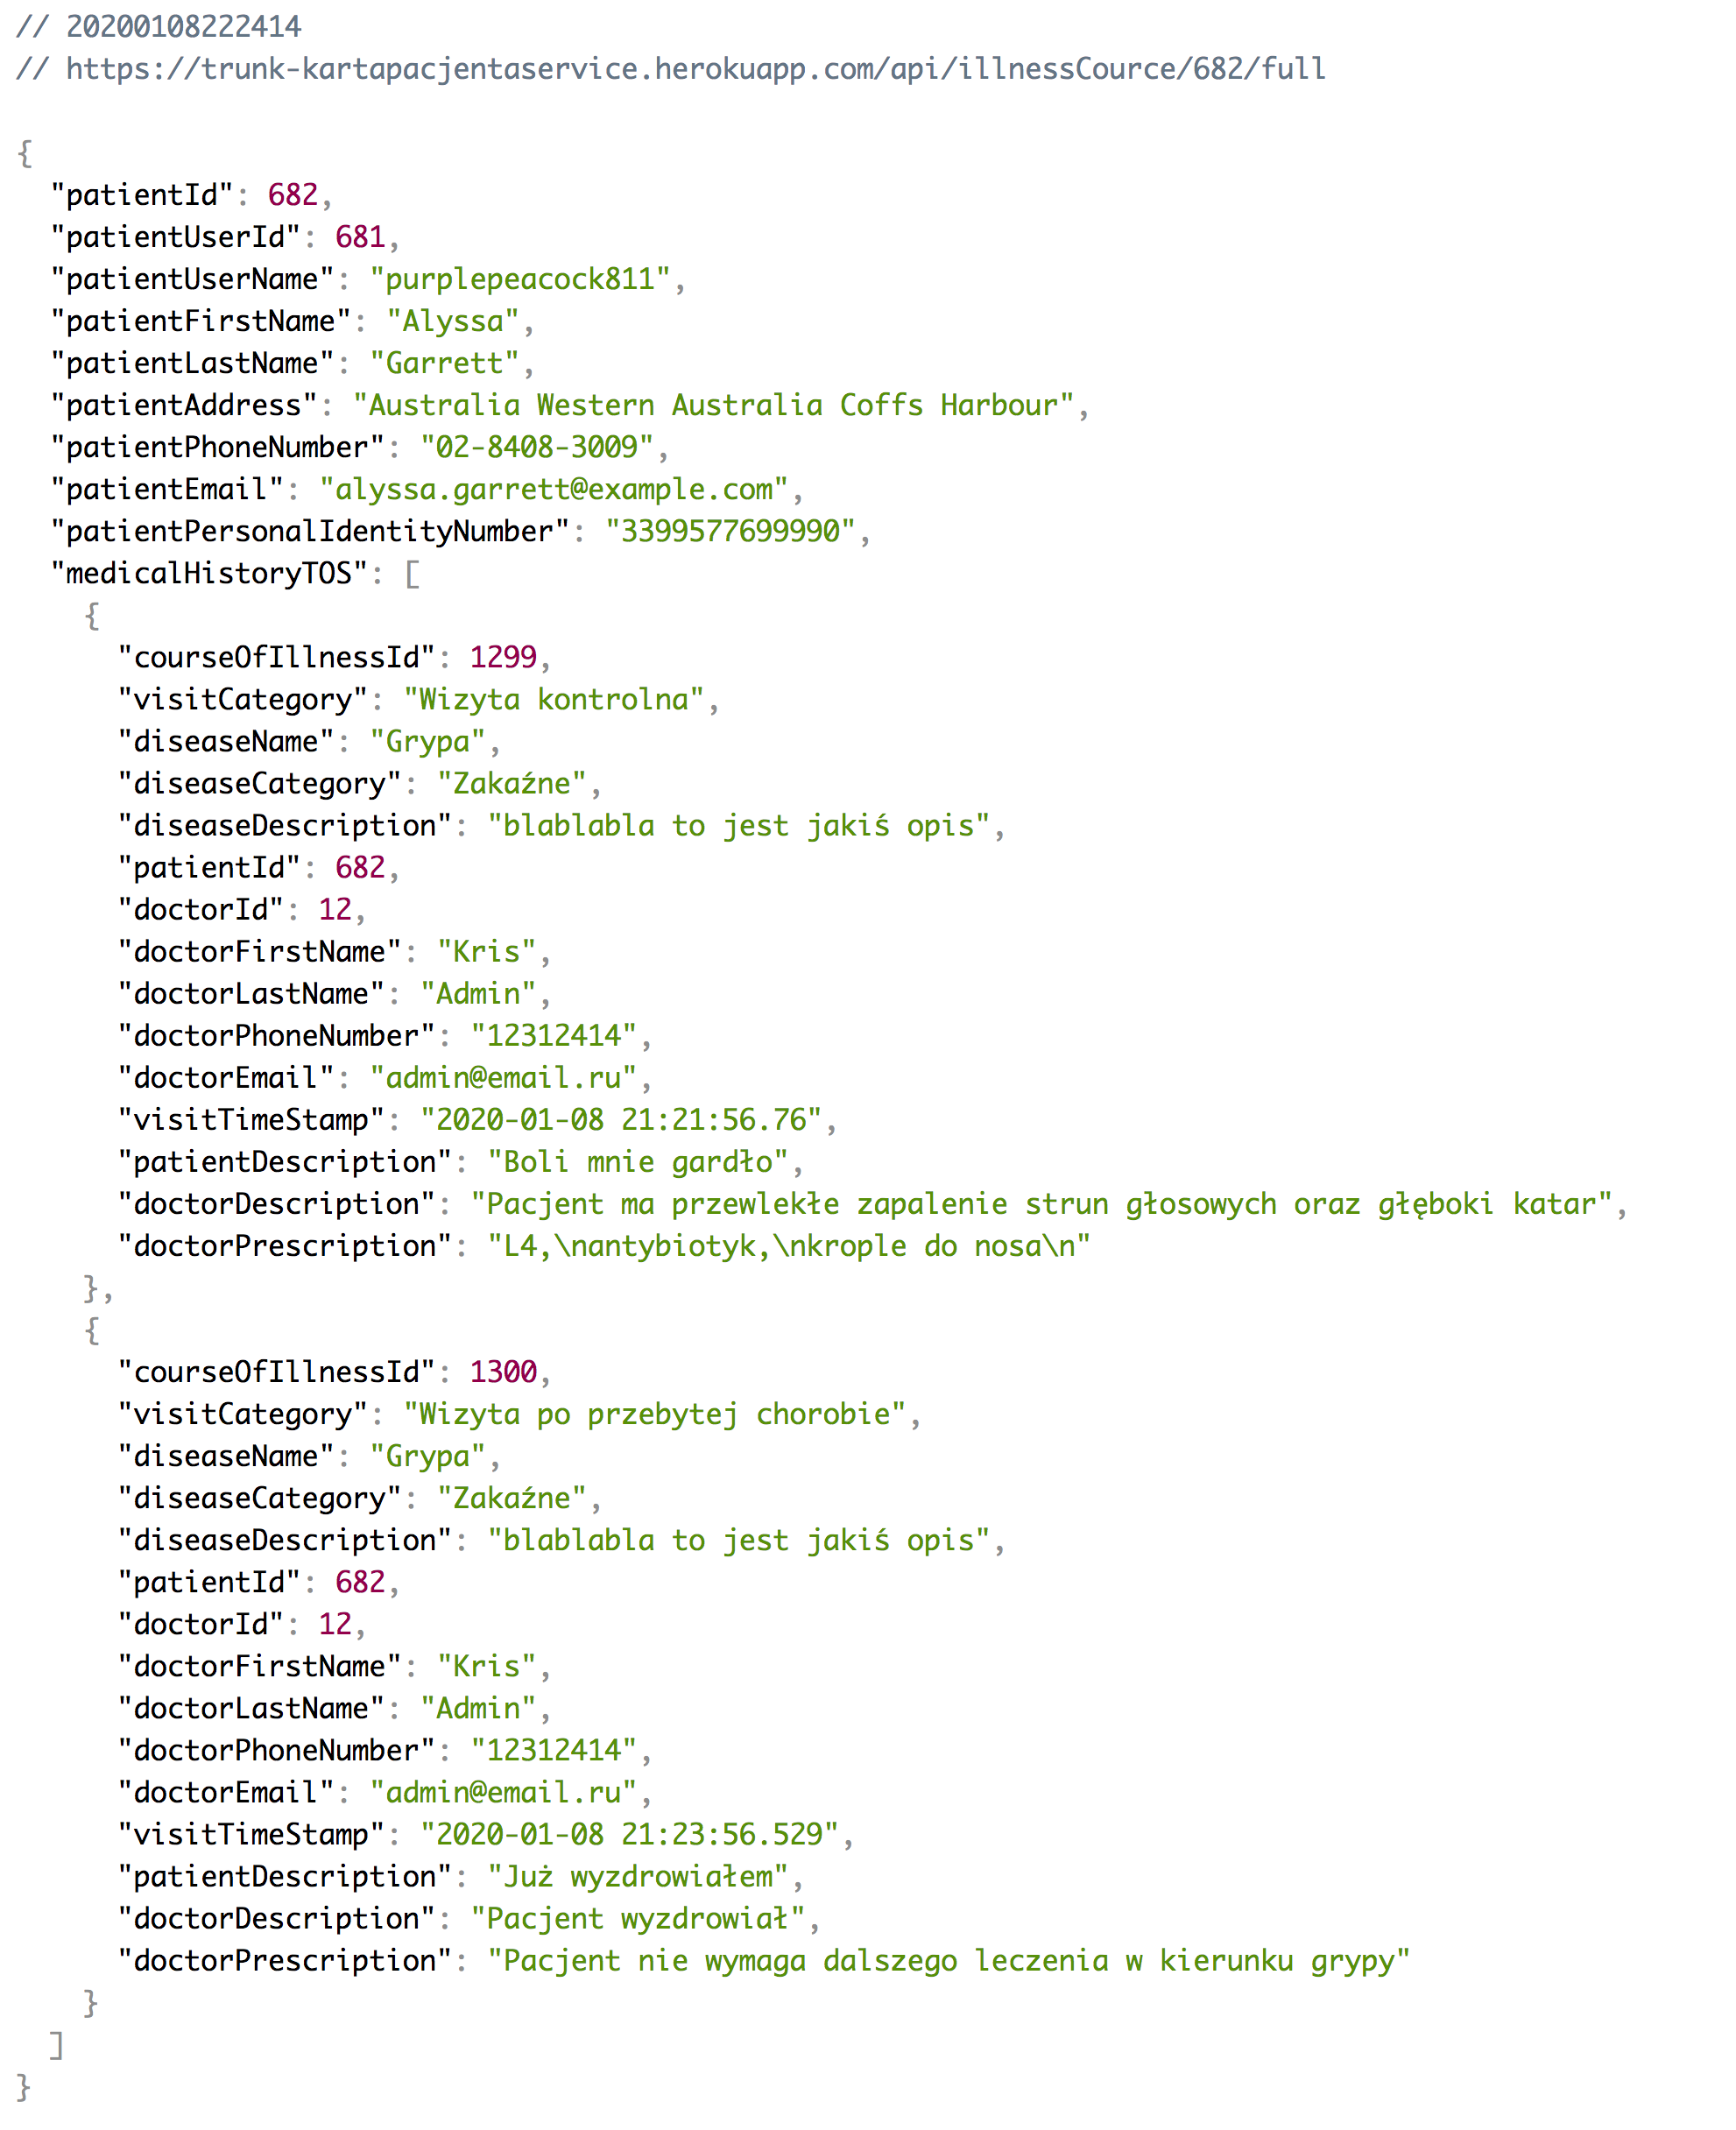
\includegraphics[width=15cm]{pictures/service/07-json_normal}
\caption{Przedstawienie pełnych danych o pacjencie i jego chorobach w formacie JSON.}
\end{figure}

% json anonim
\begin{figure}[H]
\centering
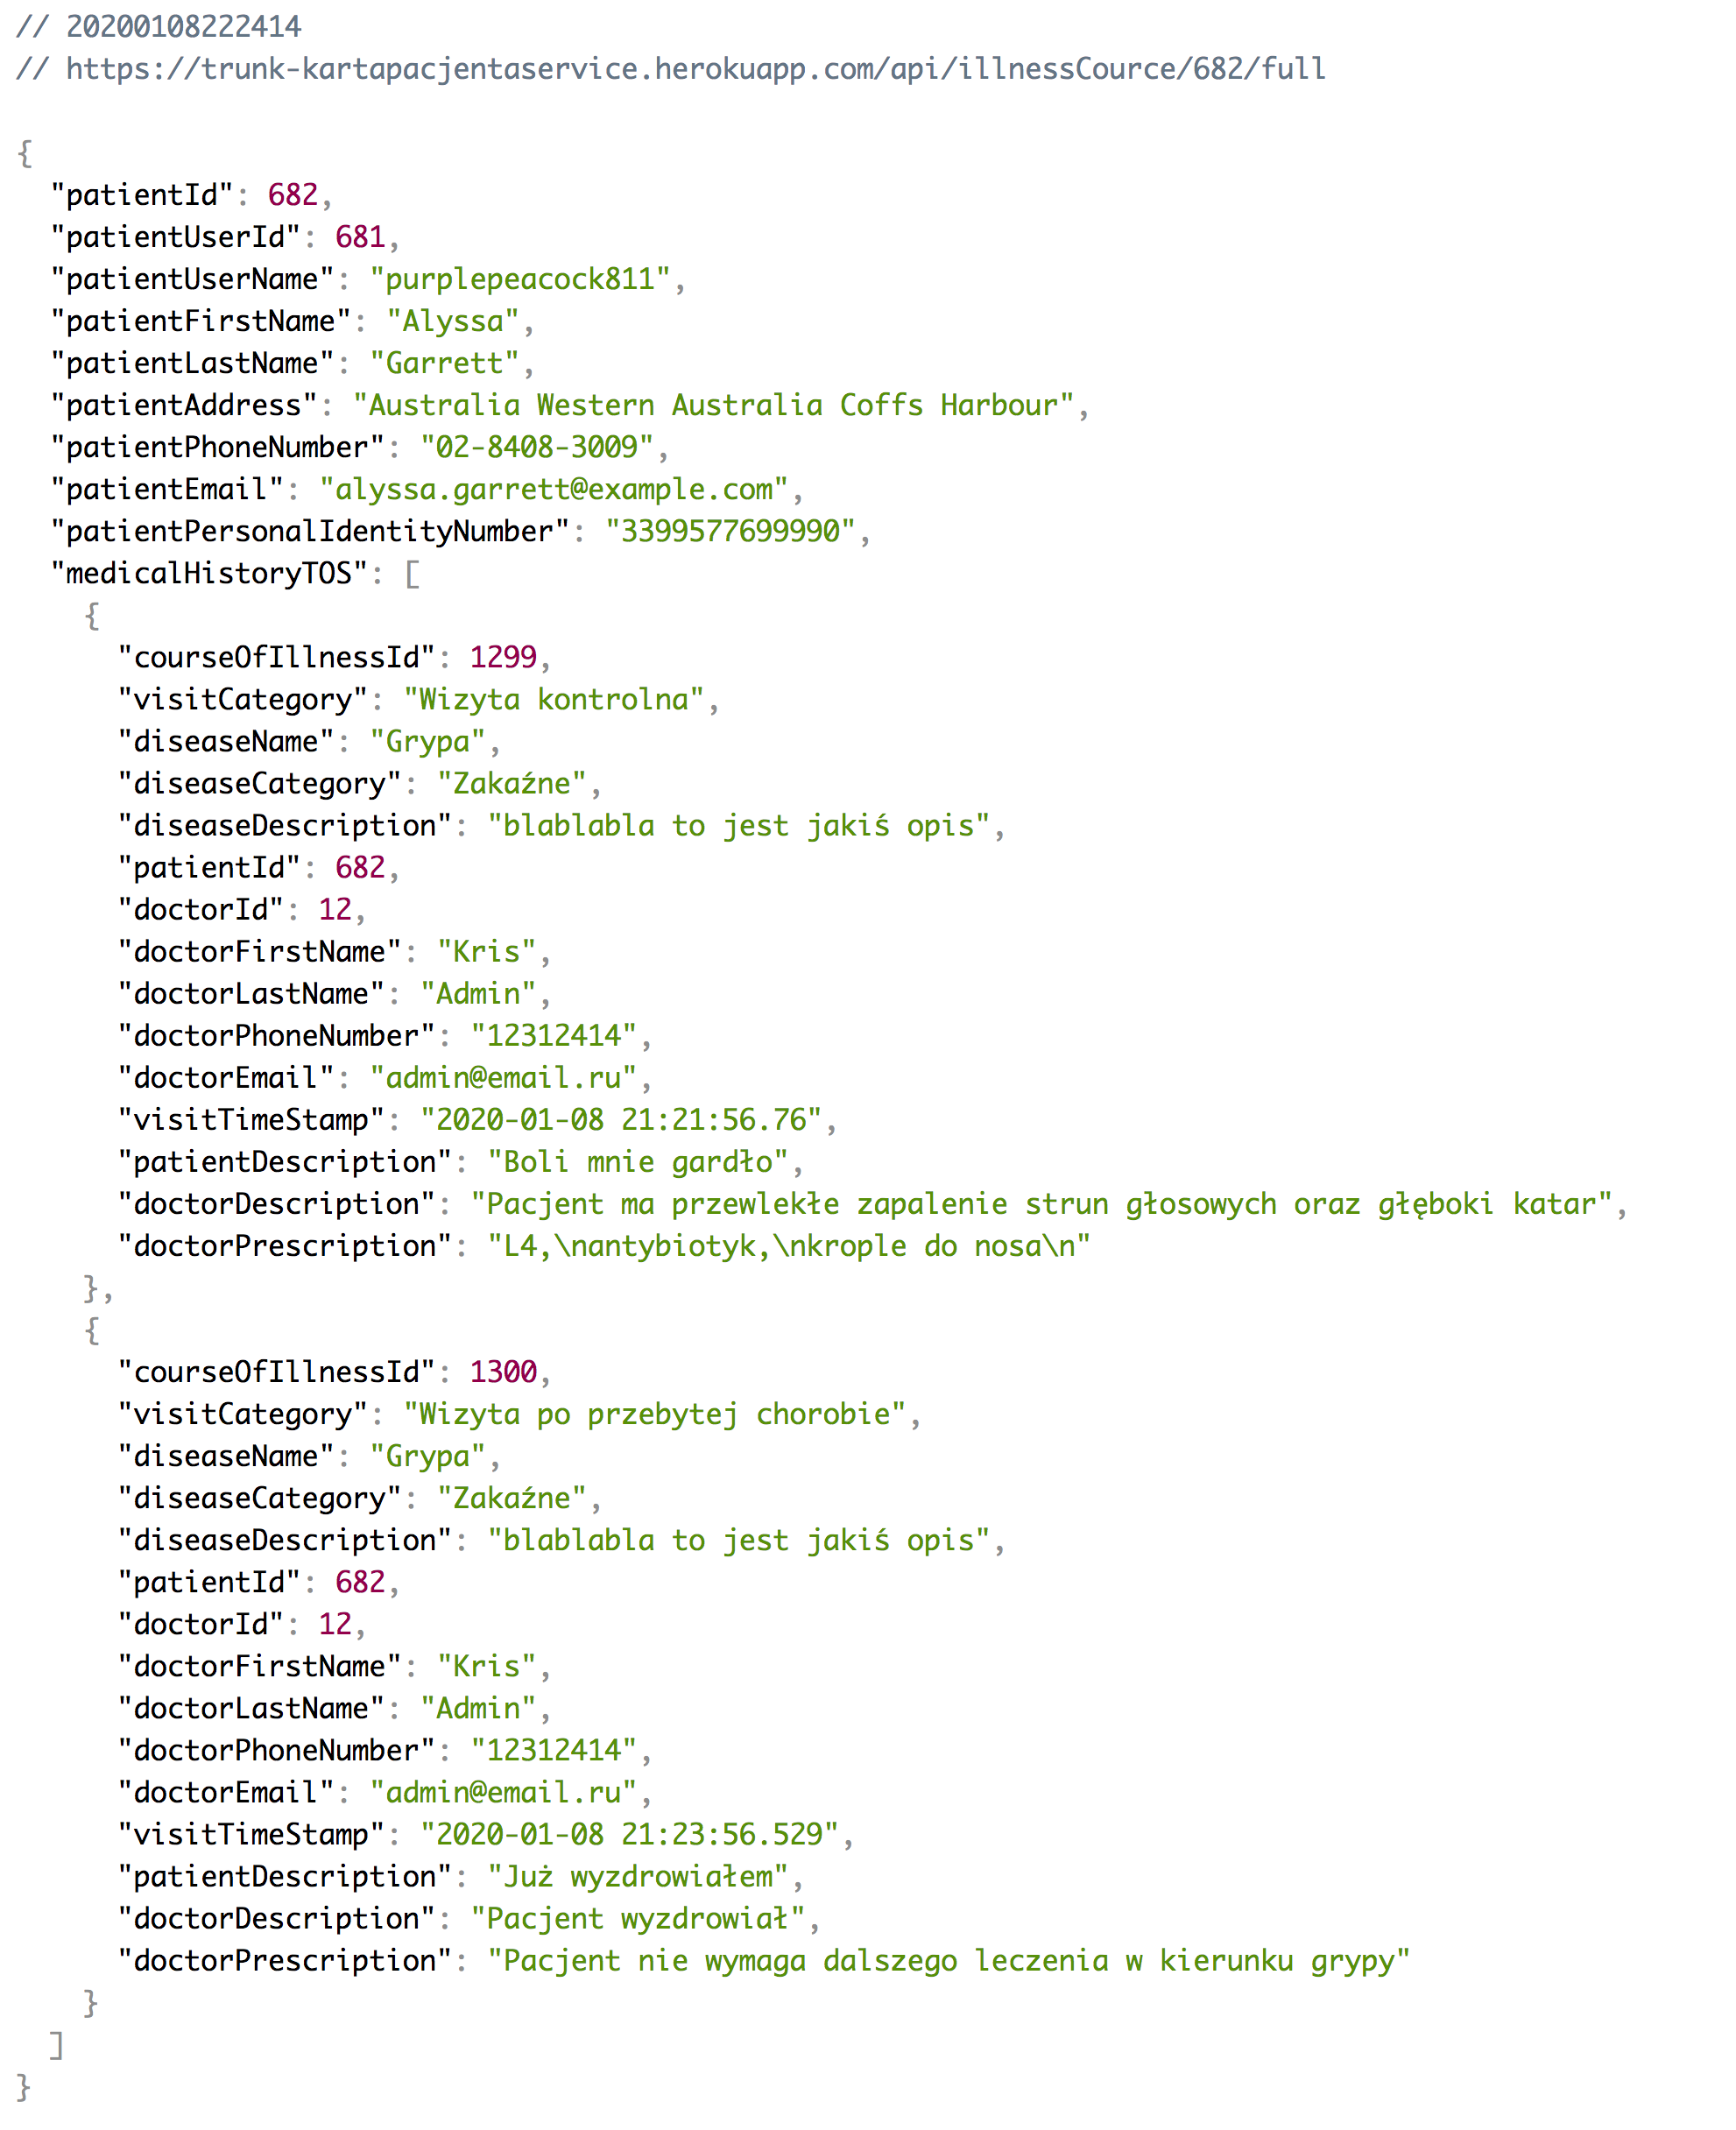
\includegraphics[width=15cm]{pictures/service/07-json_normal}
\caption{Przedstawienie anonimowych danych o pacjencie i jego chorobach w formacie JSON.}
\end{figure}

% swagger
Serwis posiada także możliwość przetestowania punktów końcowych (ang. \textit{endpoint}). Funkcjonalność dostępna jest na  \href{https://trunk-kartapacjentaservice.herokuapp.com/swagger-ui.html#/}{stronie}.

\subsection{Testowanie aplikacji}
Do przetestowania wszystkich funkcji aplikacji ,,Karta Pacjenta'' wymagane jest, aby skorzystać z konta administratora - konta różnych użytkowników posiadają różne uprawnienia. Administrator ma dostęp do wszystkich możliwych miejsc na stronie. Podczas testowania aplikacji proszę używać konta:\\
\begin{center}
\label{credentials}
login: admin\\
hasło: admin
\end{center}